\section{The CMS detector}
The overall layout of CMS is shown in \ref{fig:CMSdetector}.
At the heart of CMS apparatus sites a 4$T$ superconducting solenoid with 5.9m inner diameter. The tracker system and the calorimeters locate inside the solenoid volume which provide good momentum and energy resolution for both charged and neutral particles as well as particle identification (PID) power. The return field of superconducting solenoid is strong enough to saturate 1.5m of iron and cover the whole muon system.

\begin{figure}
    \centering
    \caption{An exploded view of the CMS detector. From Ref. \cite{cmstdr}}
    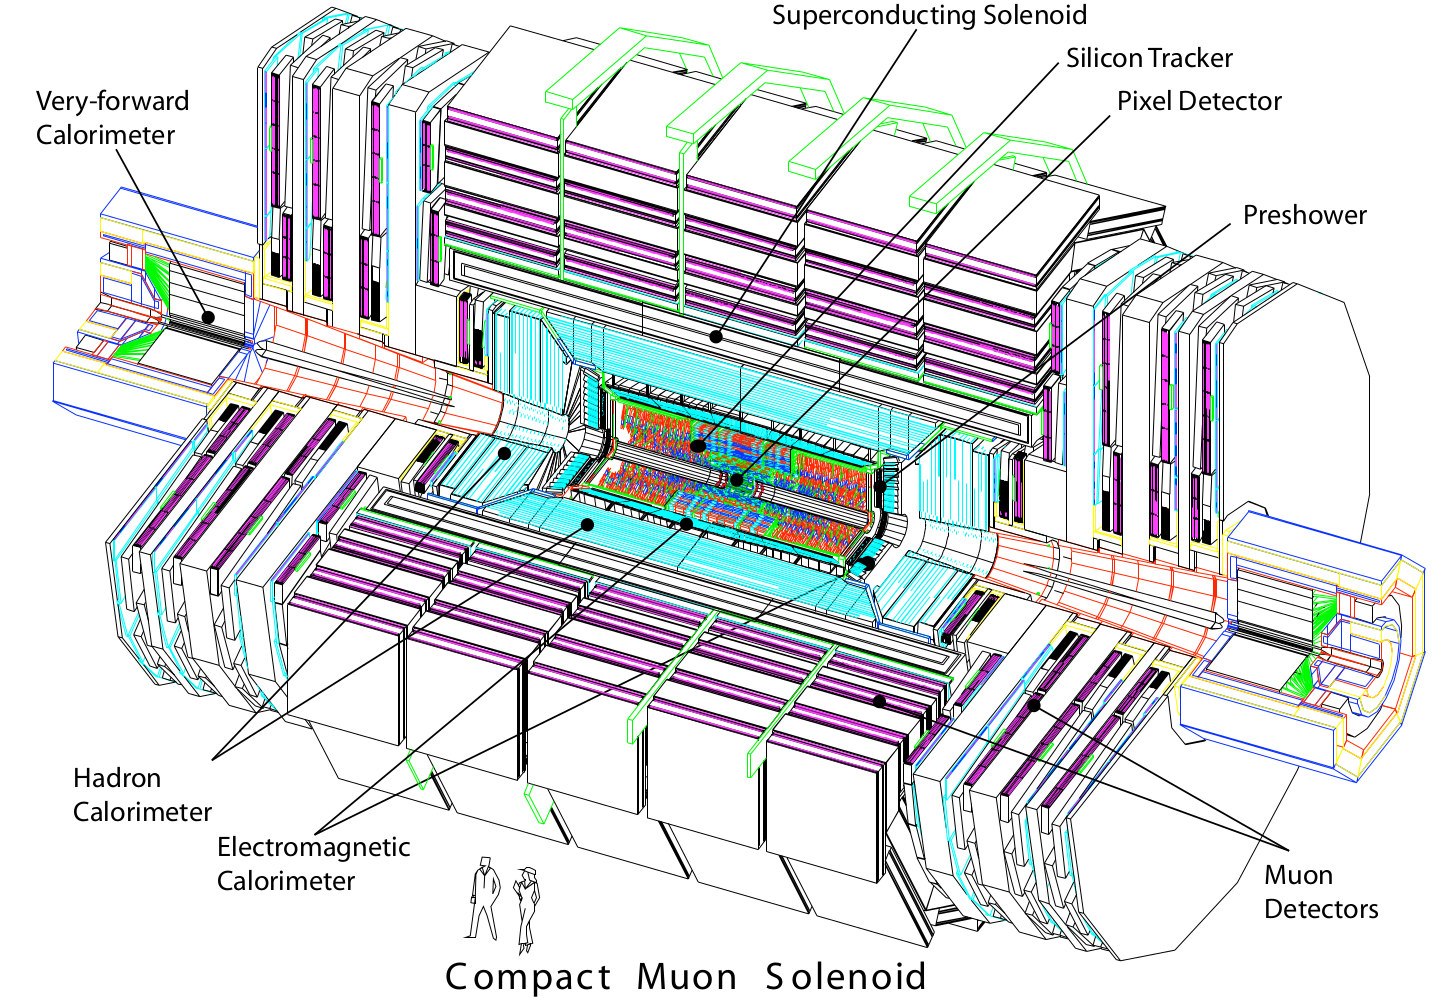
\includegraphics[width=0.5\textwidth]{fig/CMSdetector.png}
    \label{fig:CMSdetector}
\end{figure}

The magnetic field in CMS is generated by a superconducting solenoid which provides strong bending power and momentum resolution of $\Delta p/p \approx 10\% $ at $p=1TeV/c$. The parameters of the superconducting solenoid are listed in Tab.\ref{tab:magnet_parameters}:

\begin{table}[!h]
    \centering
    \caption{Parameters of the CMS superconducting solenoid. From Ref.\cite{cmstdr}}
    \begin{tabular}{|l|c|}
    \hline
    Field          &   4T      \\
    \hline
    Inner Bore     &   5.9m    \\
    \hline
    Length         &   12.9m   \\
    \hline
    Number of Turns & 2168     \\
    \hline
    Current         & 19.5kA   \\
    \hline
    Stored energy   & 2.7GJ    \\
    \hline
    Hoop stress     & 64 atm     \\
    \hline
    \end{tabular}
    \label{tab:magnet_parameters}
\end{table}

The inner tracker system is composed of silicon pixel modules placed close to the interaction region. The inner tracker is designed for high luminosity and large track multiplicities. The pixel detector are placed close to the interaction region to improve the measurement of the impact parameter as well as the position of secondary vertices. Thin silicon sensors of thickness $100-150\mu m$ are segmented into pixel size of $25 \times 100 \mu m^2$ or $50 \times 50 \mu m^2$ which provide enough radiation tolerance and deliver the desired performance in term of detector resolution, occupancy, and two-track separation. As shown in Fig. \ref{fig:tracker}, the inner tracker is composed of 4 cylindrical layers in barrel region and 8 small plus 4 large disc layers in end-cap region. The acceptance extends to  $|\eta| \approx 4$. 

The outer tracker is composed of six cylindrical barrel layers of silicon microstrip detector in the central region, covering the region of $|z|<1200mm$, complemented on each forward side by five endcap double-discs in the region of $1200 < |z| < 2700mm$. The silicon microstrip detectors provide the required granularity and precision. Modules are installed between $r \approx 21cm$ and $r \approx 112cm$. 

\begin{figure}[!h]
    \centering
    \caption{Sketch of one quarter of the tracker layout in r-z view. In the Inner Tracker the green lines correspond to pixel modules made of two readout chips and the yellow lines to pixel modules with four readout chips. In the Outer Tracker the blue and red lines represent the two types of modules described in the text. From Ref.\cite{collaboration2017phase}}
    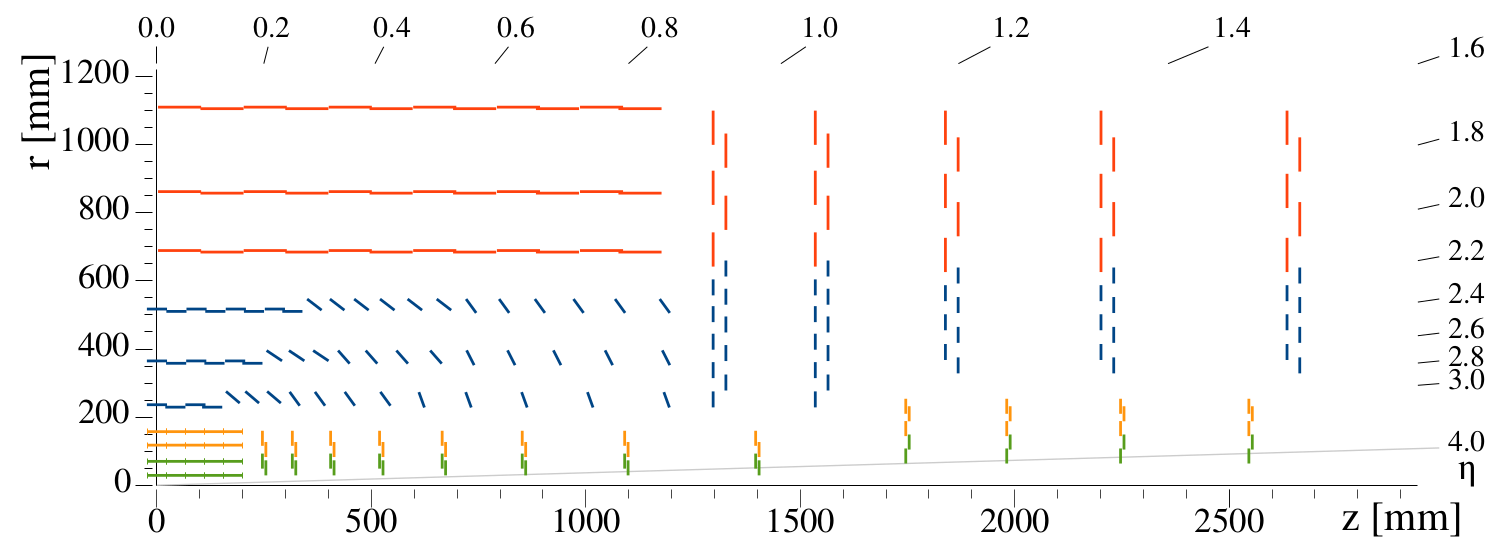
\includegraphics[width=0.5\textwidth]{fig/tracker.png}
    \label{fig:tracker}
\end{figure}

The EM calorimeter (ECAL) uses lead tungstate ($PbWO_4$) crystals with coverage in pseudorapidity up to $|\eta| < 3.0$. These crystals have short radiation ($X_0$ = 0.89 cm) and Moliere (2.2cm) lengths, short photon emission time ($80\%$ of the light is emitted within 25 ns) and radiation hard (up to 10 Mrad). The scintillation light is detected by silicon avalanche photodiodes (APDs) in the barrel region and vacuum phototriodes (VPTs) in the endcap region. The ECAL contains a barrel region and endcap region, corresponding to $0 < |\eta| < 1.479$ and $1.479 < |\eta| < 3.0$ accordingly. The crystals in the barrel section (EB) have a length of 230 mm, corresponding to 25.8 $X_0$, while the ones in the endcaps (EE) have a length of 220 mm (24.7 $X_0$). The energy resolution of ECAL can be parameterized as a function of energy: 

\begin{equation}
    (\frac{\sigma}{E})^2 = (\frac{S}{\sqrt{E}})^2 + (\frac{N}{E})^2 + C^2
\end{equation}

where $S$ is the stochastic term term, $N$ is the noise and the $C$ the constant. The values of these parameters are listed in the figure.

\begin{figure}[!h]
    \centering
    \caption{ECAL supermodule energy resolution, $\sigma_E/E$, as a function of electron energy as measured from a beam test. From Ref.\cite{cmstdr}}
    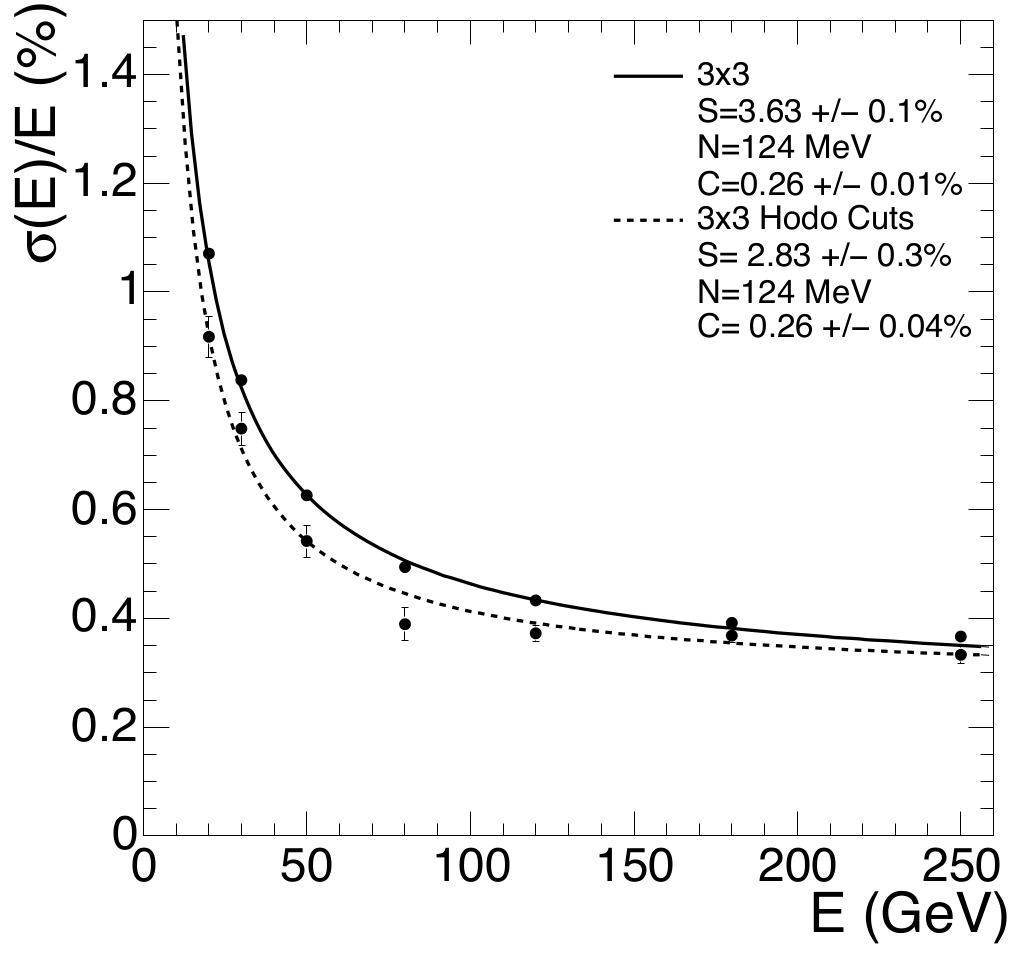
\includegraphics[width=0.45\textwidth]{fig/energyresolution.png}
    \label{fig:energyresolution}
\end{figure}

The ECAL is surrounded by a brass/scintillator sampling hadron calorimeter (HCAL) with coverage up to $|\eta | < 3.0$. The scintillation light converted by wavelength-shifting (WLS) fibres embedded in the scintillator tiles and channeled to photodetectors via clear fibres. The photons are detected by hybrid photodiodes (HPDs) that can provide gain and operate in high axial magnetic fields. The central calorimetery is complemented by a "tail-catcher" in the barrel region which extend the material length to 11 hadronic interaction length $\lambda_I$. The thickness in interaction lengths varis from $7-11 \lambda_I$ for HCAL depending on $\eta$. Coverage between pseudorapidities of 3.0 and 5.0 is provided by the steel/quartz fibre Hadron Forward (HF) 

The muon system (MS) containing 4 muon "stations". The layout of muon system is shown in fig. \ref{fig:muonsystem} Each station consists of several layers of aluminum drift tubes (DT) in the barrel region and cathode strip chambers (CSCs) in the endcap region, complemented by resistive plate chambers (RPCs) in  both region. In the barrel region ($|\eta| < 1.2$), where the muon rate is low and the residual magnetic field in the chambers is low, DT chambers are used. In endcap region, where the muon rate and magnetic field are high, CSC are deployed and cover the region up to $|\eta| < 2.4$.

\begin{figure}[!h]
    \centering
    \caption{Layout of one quarter of the CMS muon system for initial low luminosity running. THe RPC system is limited to $|\eta| < 1.6$ in the endcap, and for the CSC system only the inner ring of the ME4 chambers have been deployed. From Ref.\cite{cmstdr}}
    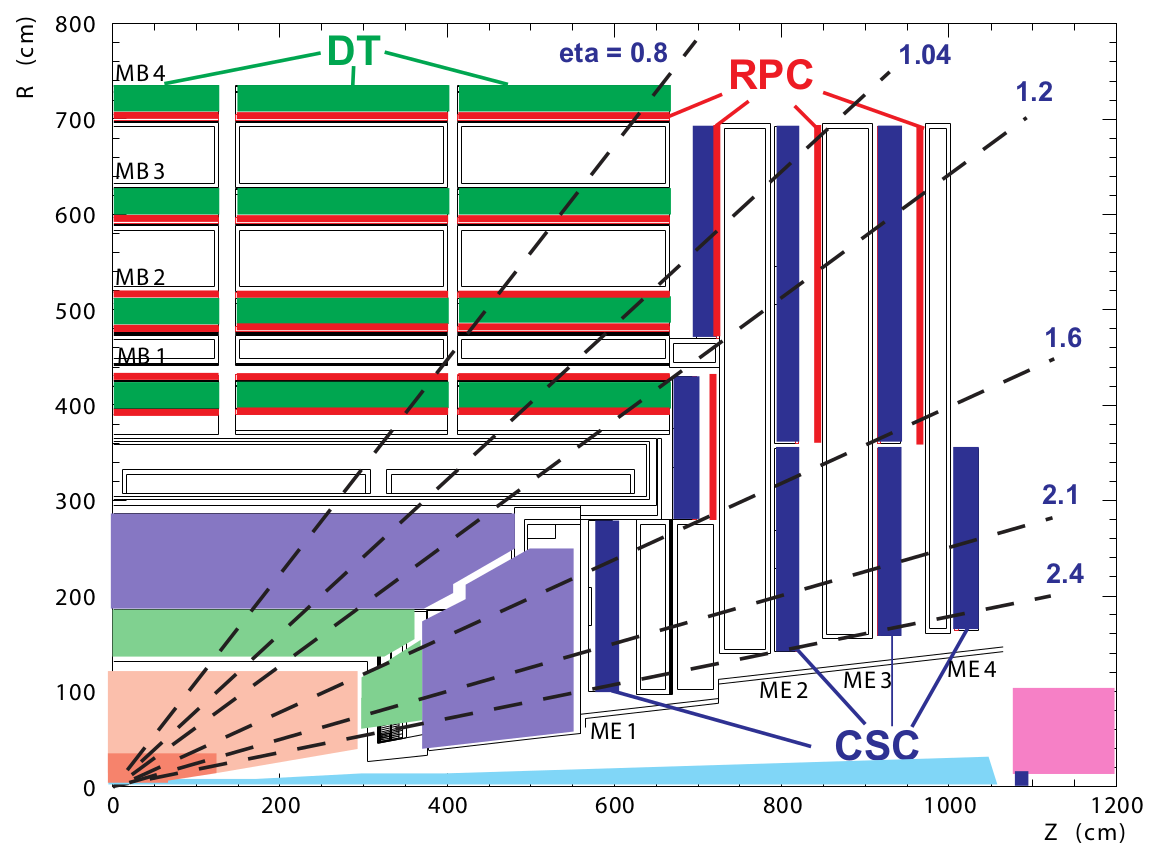
\includegraphics[width=0.5\textwidth]{fig/muonsystem.png}
    \label{fig:muonsystem}
\end{figure}

The CMS trigger and data acquisition system consists 4 parts: the detector electronics, the Level-1 (L1) trigger processors, the readout network, and an online event filter system for High-Level Trigger (HLT). The L1 triggers contains the calorimetry and muon system as well as some correlation of information between systems. The L1 decision is based on the presence of "trigger primitive" objects e.g. photons, electrons, muons and jets passing $E_T$ or $p_T$ thresholds. Reduced-granularity and reduced-resolution data are used to reconstruct trigger objects. Global sum of $E_T$ and $E_T^{miss}$ are also employed for global trigger.  The design value of L1 rate is 100 kHz by the average time to transfer full detector information through the readout system. The event selection at the HLT using reconstructed objects and identification criteria to select events with possible interest for data analysis. The HLT hardware consists of the event filter farm (EVF) composed of commodity computer. The filtering process uses the full precision of the data from the detector, and the selection is based on offline-quality reconstruction algorithms. The data processing of the HLT is structured around the concept of a HLT path, which is a set of algorithmic processing steps run in a predefined order that both reconstructs physics objects and makes selections on these objects. HLT reduce the the L1 output rate of 100 kHz to order of 1kHz for massive storage.

A more detailed description of the CMS detector can be found in  \cite{adolphi2008cms}
